\documentclass{article}
\usepackage{tikz}
\usetikzlibrary{arrows.meta,positioning,calc,shapes.geometric}
\pagestyle{empty}
\begin{document}
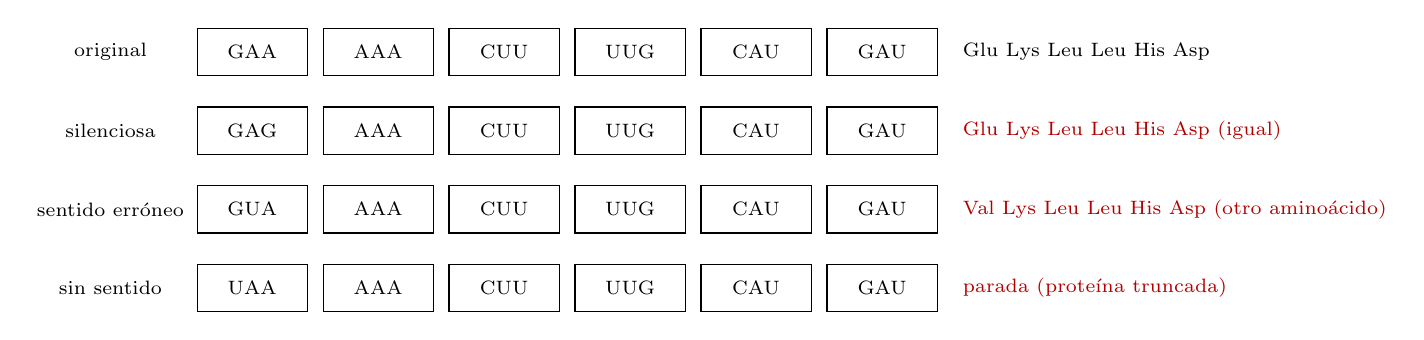
\begin{tikzpicture}

\node[font=\scriptsize] at (-1.8,3.0) {original}; \node[font=\scriptsize] at (-1.8,2.0) {silenciosa}; \node[font=\scriptsize] at (-1.8,1.0) {sentido erróneo}; \node[font=\scriptsize] at (-1.8,0.0) {sin sentido};
\foreach \y/\a/\b/\c/\d/\e/\f in {3.0/GAA/AAA/CUU/UUG/CAU/GAU, 2.0/GAG/AAA/CUU/UUG/CAU/GAU, 1.0/GUA/AAA/CUU/UUG/CAU/GAU, 0.0/UAA/AAA/CUU/UUG/CAU/GAU} {
  \foreach \x/\t in {0/\a,1.6/\b,3.2/\c,4.8/\d,6.4/\e,8.0/\f} {\node[draw, minimum width=1.4cm, minimum height=0.6cm, font=\scriptsize] at (\x,\y) {\t};}}
\node[font=\scriptsize, right] at (8.9,3.0) {Glu Lys Leu Leu His Asp};
\node[font=\scriptsize, right, red!70!black] at (8.9,2.0) {Glu Lys Leu Leu His Asp (igual)};
\node[font=\scriptsize, right, red!70!black] at (8.9,1.0) {Val Lys Leu Leu His Asp (otro aminoácido)};
\node[font=\scriptsize, right, red!70!black] at (8.9,0.0) {parada (proteína truncada)};

\end{tikzpicture}
\end{document}
